
\documentclass{tufte-handout}

\usepackage{amsmath}
\usepackage{graphicx}

\title{Single Partition Regression Analysis}
\author{Rhys Hawkins and Malcolm Sambridge}

\usepackage{units}

\usepackage{fancyvrb}
\fvset{fontsize=\tiny}

\usepackage{listings}
\lstset{basicstyle=\tiny, numbers=left, frame=single, language=Python}

\begin{document}

\maketitle

\begin{abstract}

This tutorial describes how to analyse continuous data using Monte-Carlo
Markov-Chain based regression.

\end{abstract}

\section{Pre-requisites}

This tutorial is for the Python version of the rjmcmc library. The examples
rely on the Matplotlib library for plotting. The versions used in the 
development of this tutorial are as follows:

\begin{itemize}
\item Python 2.7.1
\item rjmcmc 0.1.0
\item Matplotlib 1.1.0
\end{itemize}

\section{The Data}

For this tutorial we will use a non-trivial (in the sense that it will
require a higher order polynomial to fit the function correctly)
synthetic dataset with added noise.

The function that is used is an exponentially increasing sine wave over 
the domain 0 $\ldots$ 10, ie:

\begin{equation}
y = e^\frac{x}{3} \sin{ \frac{2x}{3}}
\end{equation}

\begin{marginfigure}
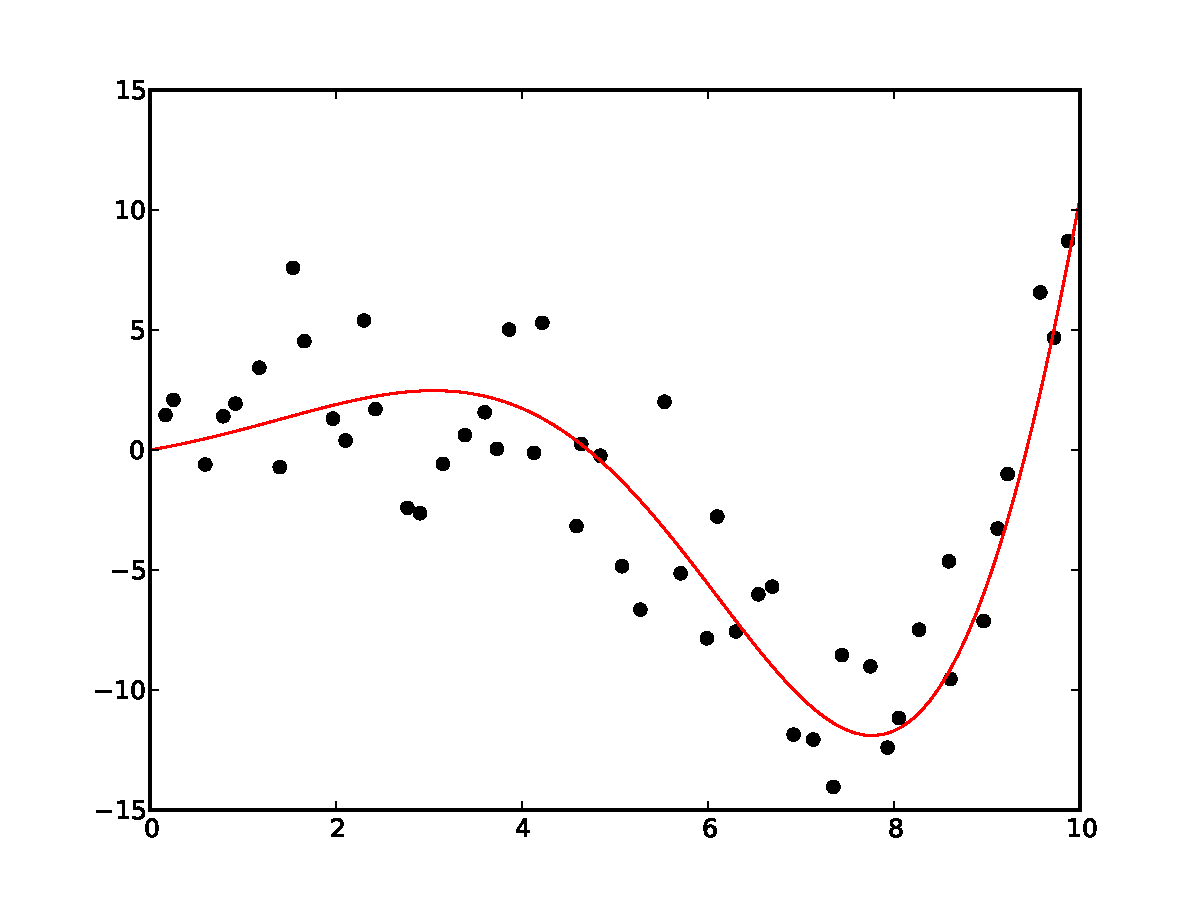
\includegraphics[width=\linewidth]{../ch0-exampledata.pdf}
\caption{The Synthetic Data.}
\label{fig:syntheticdata}
\end{marginfigure}

The actual dataset unevenly (though with fairly good coverage) samples
this function and adds some Gaussian noise and these values are save
to an ASCII text file. A plot of the synthetic data points with the 
true function is shown in Figure~\ref{fig:syntheticdata}.

\section{Loading the Data}

For those unfamiliar with Python, we discuss briefly the loading of data
from a simple ASCII text file. The code for loading the data and doing
a simple plot is shown in Listing~\ref{lst:loadingdata}.

\lstset{caption=Loading the Data.,label=lst:loadingdata}
\lstinputlisting{../ch1-loading.py}

The ASCII file contains an x, y pair per line separated by a space. On
line 12, we use the built in function {\tt open} to open the file. One
lines 15 and 16 we initialize 2 list that will contain the x and y 
coordinates in the file. On line 18 we loop through the lines in the 
file and add each x, y pair to the 2 separate lists.

\begin{marginfigure}
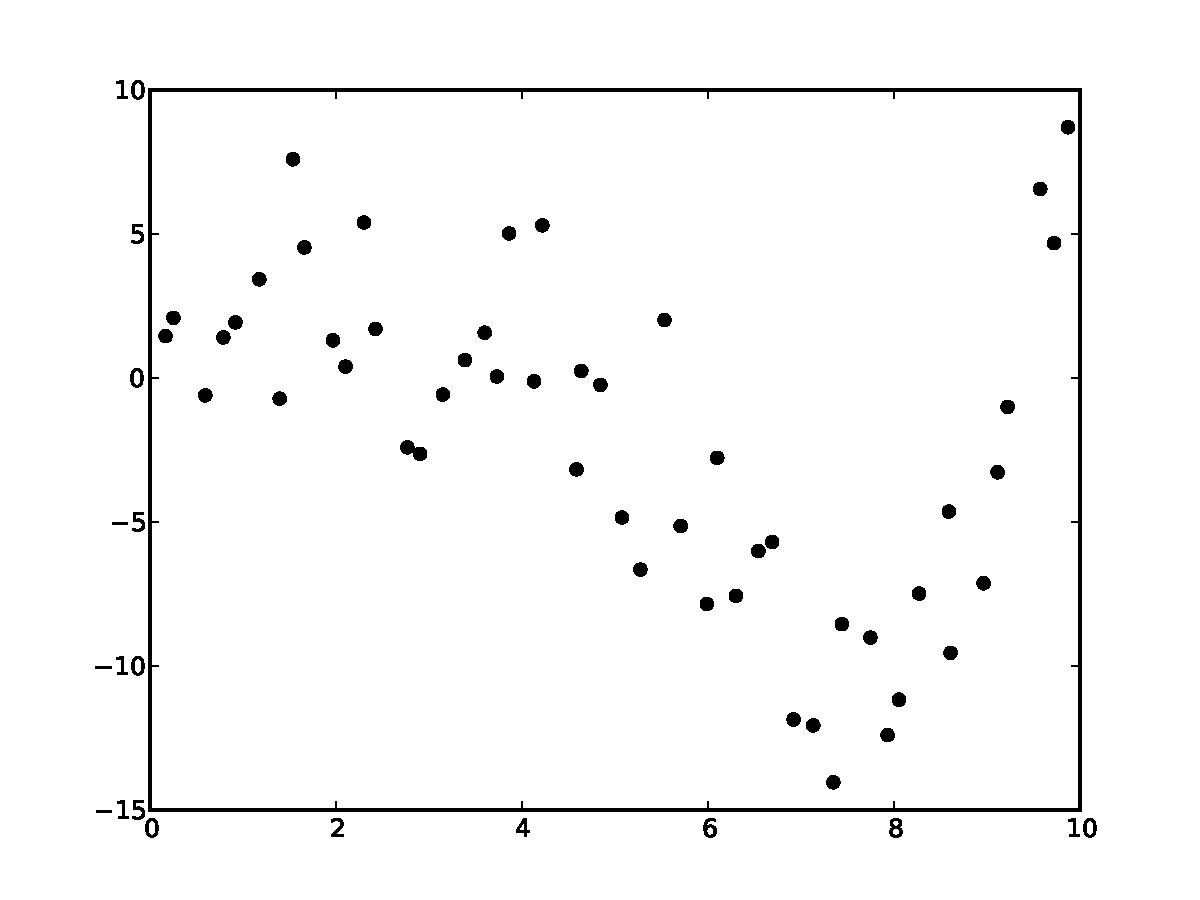
\includegraphics[width=\linewidth]{../ch1-loading.pdf}
\caption{Noisy data and true curve used in test problem.}
\label{fig:loading}
\end{marginfigure}

From line 26 onwards, we plot the data using the matplotlib library
and save the plot to a PDF file. The plot resulting from this script
can be seen in Figure~\ref{fig:loading}.

\section{Running the default analysis}

For performing an regression analysis on a continuous dataset the function is called
{\tt regression\_single1d}. The parameters for this function are as follows with 
default values shown where applicable:

\begin{description}
\item[dataset] The dataset object to run the analysis on. This is an rjmcmc.dataset1d
object which wraps the x and y vectors you load from the file and includes individual
point noise values. This is the only parameter which doesn't have a default value.
\item[burnin = 10000] The number of initial samples to throw away.
\item[total = 50000] The total number of samples to use for the analysis.
\item[max\_order = 2] The maximum order of polynomial to use to fit the data.
\item[xsamples = 100] The number of points to sample along the x direction for the curve.
\item[ysamples = 100] The number of points to sample along the y directory for the statistics such
as mode, median and confidence intervals. This is the number of bins for the histograms in the 
y direction.
\item[confidence\_interval = 0.95] The confidence interval to use for minimum and maximum confidence
intervals. This should be a value between 0 and 1.
\end{description}

For this analysis we are only going to use the default values and the listing is shown in 
Listing~\ref{lst:defaultanalysis}. 

\lstset{caption=Running the Default Analysis.,label=lst:defaultanalysis}
\lstinputlisting{../ch2-analyse.py}

The preamble (lines 1 $\ldots$ 24) consists of loading the file as in the previous
section. 

An important part of the analysis is estimating the error in the data.
This is specified as a error value per data point and can be thought of a weighting
as to how well the fit will attempt to fit an individual point. If the value
is low, then the fit will be tight and conversely if the value is high then the 
fit will be loose. On lines 29 and 30 we set a value of 3.0 for all data points.
Use this value for now, but try other values greater than 0.0 to see the effect.

On line 35 we construct the dataset1d object from the x, y and n lists we created.
These lists must be the same length.

On line 40 we run the analysis with this dataset1d object. The regression\_single1d
function returns a resultset1d object which contains various results and diagnostics
about the analysis. For this simple analysis we simply take the x sampling coordinates
and the mean of the fits. And plot the mean with the original data points to see 
how representative the mean is. This plot is shown in Figure~\ref{fig:defaultanalysis}.

\begin{marginfigure}
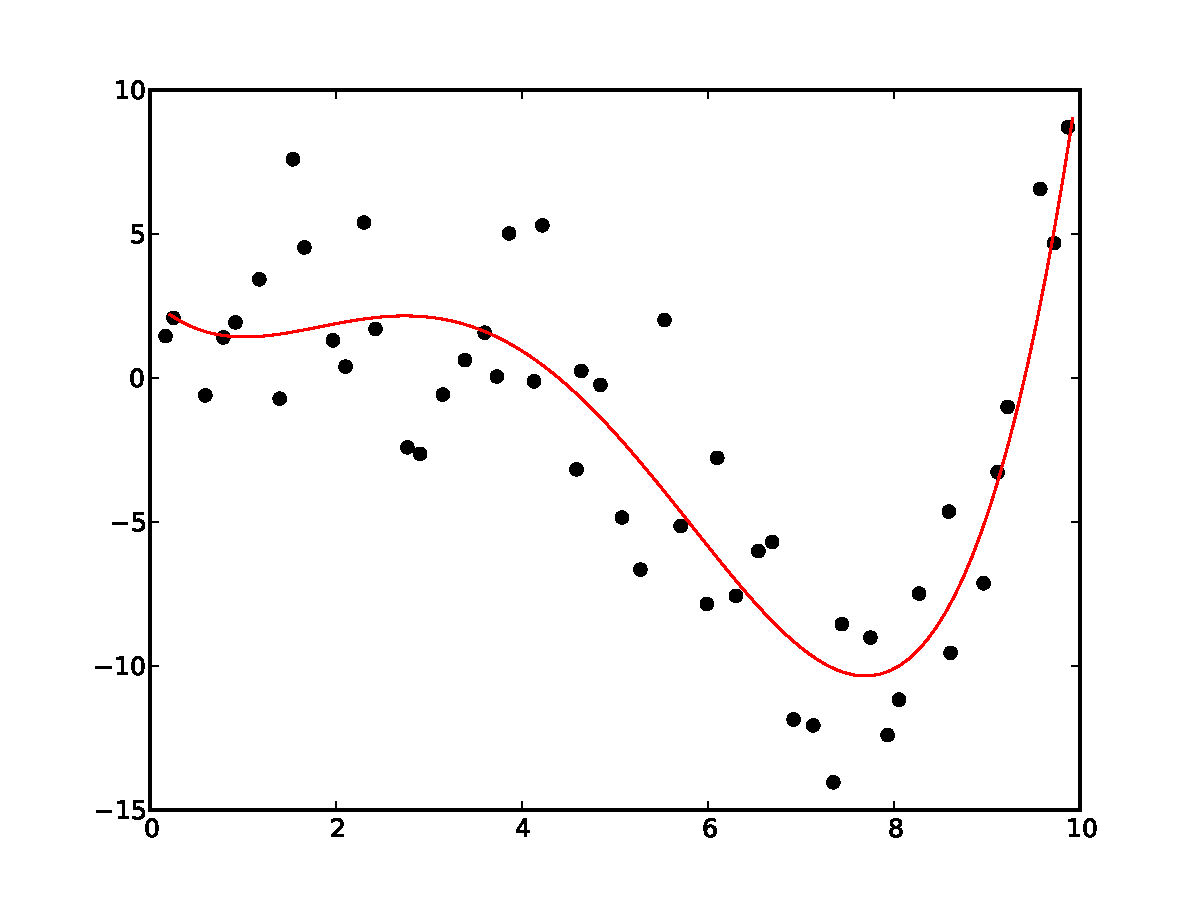
\includegraphics[width=\linewidth]{../ch2-analyse.pdf}
\caption{The Default Analysis Plot.}
\label{fig:defaultanalysis}
\end{marginfigure}

\section{Order Analysis}

A question we may ask is what order best represents the underlying
function. We can develop some understanding of this by constraining
the maximum allowable order of the fit and observing when the order
histogram converges and/or the mean of the fits converges. The script
to do this for this dataset is shown in
Listing~\ref{lst:orderanalysis}.

\lstset{caption=Order Analysis.,label=lst:orderanalysis}
\lstinputlisting{../ch3-orderanalysis.py}

In lines 41 $\ldots$ 46 we set some parameters and run several
analyses with different allowed maximum polynomial order and store
the results.

In lines 51 $\ldots$ 78 we plot the mean of the fits for each of the
constrained analyses. This plot is shown in
Figure~\ref{fig:orderanalysis}.  As can be seen from this plot, there
is very little difference between the Max. Order 3, 4, 5 curves which
implies that the data is cubic.

\begin{figure}
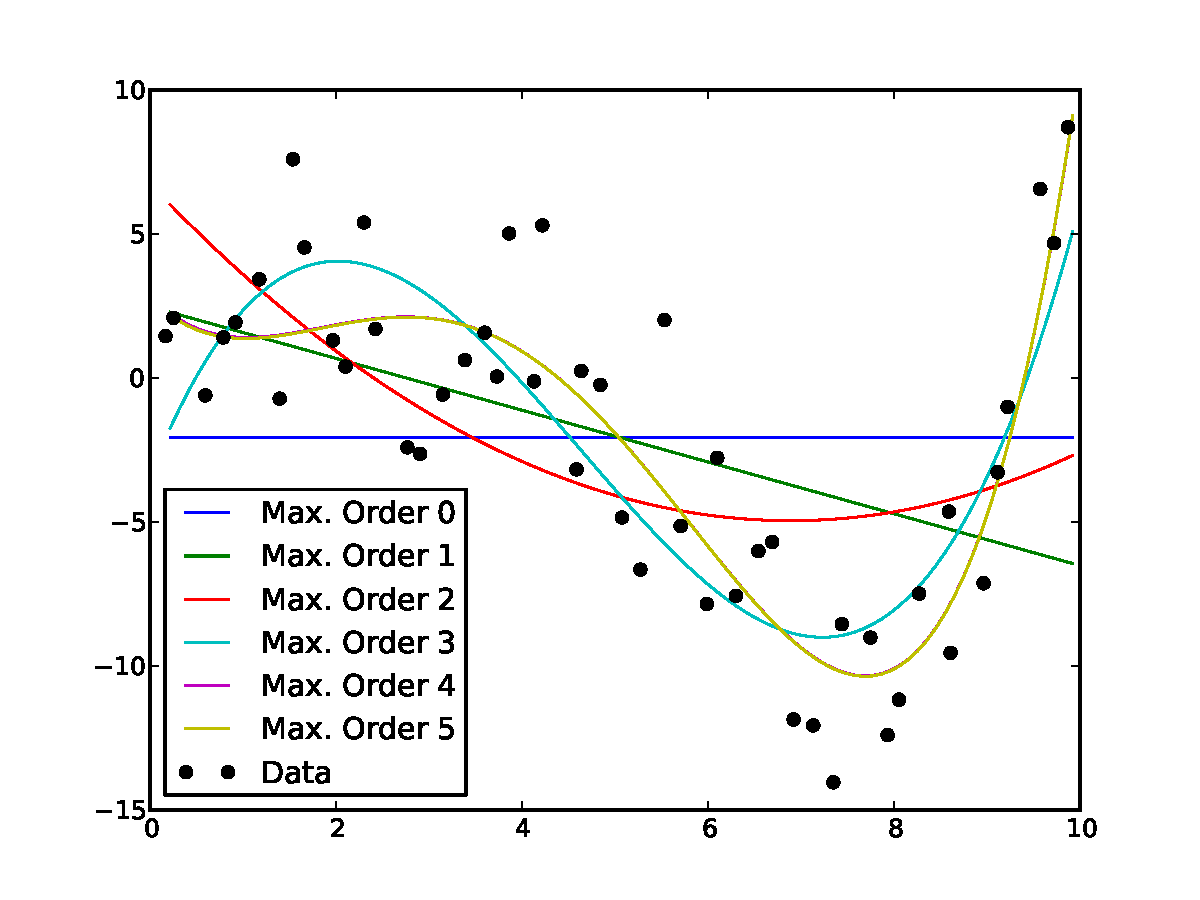
\includegraphics[width=\linewidth]{../ch3-orderanalysis.pdf}
\caption{The Mean Curves for different maximum orders.}
\label{fig:orderanalysis}
\end{figure}

In lines 80 $\ldots$ 99 we plot the progression of the order 
histogram. The order histogram reports the count of polynomials
of each order where the order is randomly choosen from a 
probability distribution determined by the data itself. This 
plot is shown in Figure~\ref{fig:orderanalysishist}.

\begin{figure}
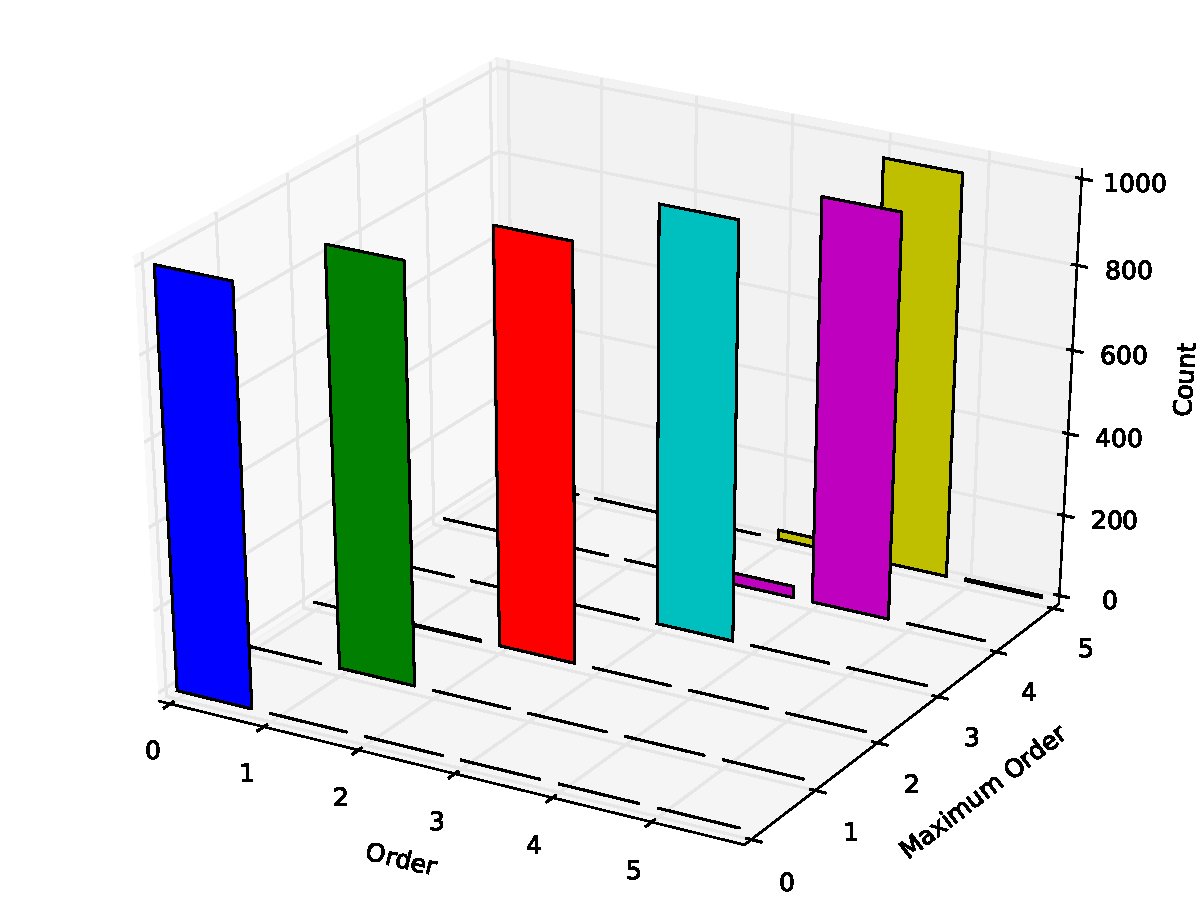
\includegraphics[width=\linewidth]{../ch3-orderanalysishist.pdf}
\caption{Posterior PDFs of the polynomial order parameter as a function of maximum allowed order.}
\label{fig:orderanalysishist}
\end{figure}

Looking at the figure, it can be seen that when the maximum permitted
order is 0, all the curves sampled are 0th order as expected. As this
maximum order is increased, the distribution of orders changes until
the step from 4 to 5 where there is little difference. It should be
noted that if a tighter noise parameter is used, that this will change
slightly as higher order polynomials will be more favoured to fit the
data better.

\section{Confidence Intervals}

So far we have only plotted the mean of the fits, however this gives
us no indication of distribution of the fit (this can be thought of as
the confidence of the fit). There are a number of ways in which we can
look at this and one of these is to look at the curves generated
during the analysis. The listing to do this is in
Listing~\ref{lst:confidence}.

\lstset{caption=Confidence Intervals., label=lst:confidence} 
\lstinputlisting{../ch4-confidence.py}

In this script we call a slightly different function called {\tt
  regression\_single1d\_sampled} which accepts a callback function.
We define this function on lines 46 $\ldots$ 55. This function 
accepts an x and y list which is the discretization of the current 
fitting polynomial being used. In this function we sample every
5th polynomial and store them. 

On lines 70 $\ldots$ 90 we plot the data as black dots, and
the mean fit with a red line over plots of all the fits we sampled.
This plot is shown in Figure~\ref{fig:confidence}.

\begin{figure}
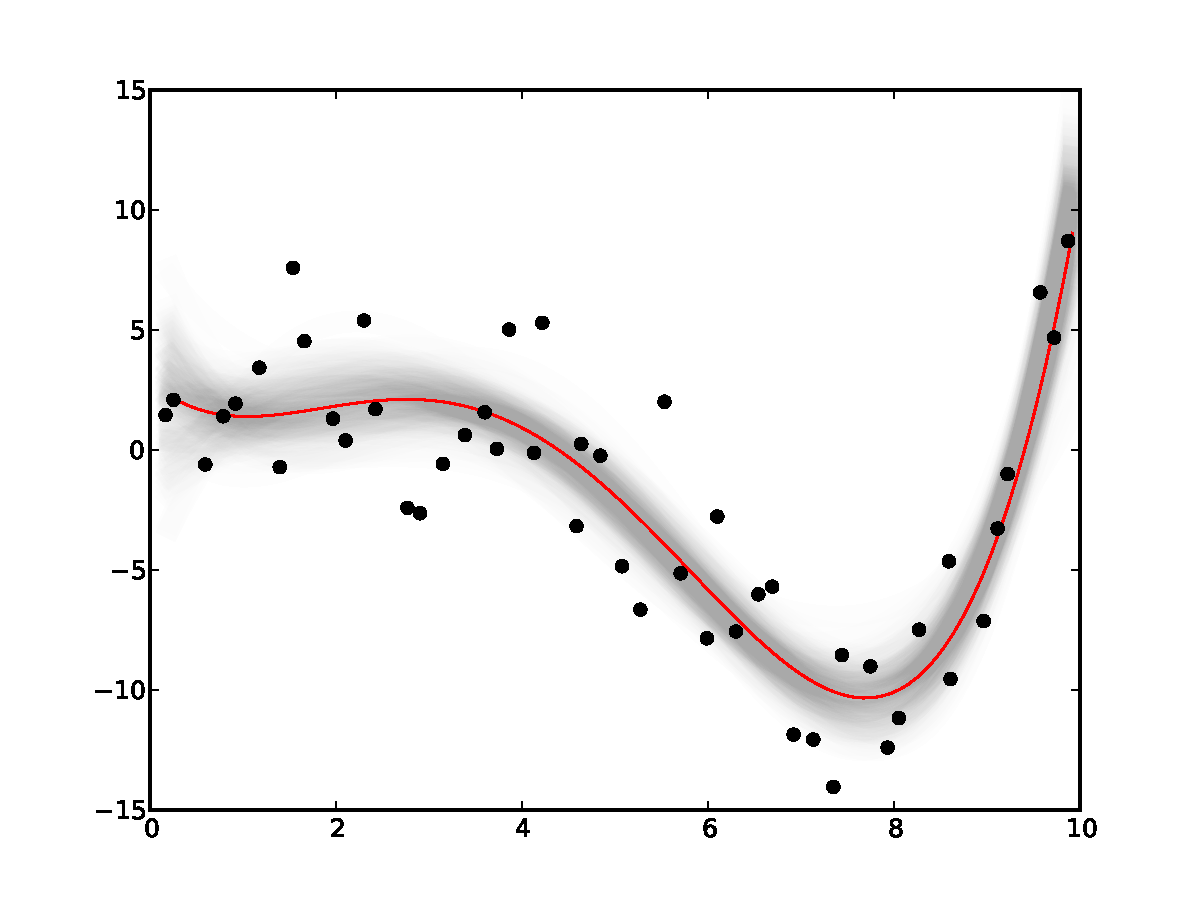
\includegraphics[width=\linewidth]{../ch4-confidence.pdf}
\caption{Sampled Confidence Intervals.}
\label{fig:confidence}
\end{figure}

The sampled fits are plotted with transparency so that where they
overlap this will show increased density implying that where these
sampled polynomial ensemble appears darker, we can have higher 
confidence that the underlying function passes through that
region.

\section{Estimating data noise}

With the hierarchical Bayesian approach we include the standard deviation
of the noise on the observations as an unknown. In the above examples
the noise $\sigma$ was set to 3 units, but the actual $\sigma$
of the data noise in Figure 1 is 2.5.
Can we use the data to detect the true standard deviation of its noise?
The hierarchical Bayesian sampling scheme is implemented with the script 
in Listing~\ref{hierarchical}. Inference on the noise is implemented by 
introducing a new parameter, $\lambda = \frac{\sigma_{est}}{\sigma_{true}}$, 
defined as the ratio of the estimated noise to the real noise.

\lstset{caption=Hierarchical Bayesian sampling to determine the data noise standard deviation, label=hierarchical} 
\lstinputlisting{../ch5-hierarchical.py}

In this script we set up a uniform prior on $\lambda$ over a pre-determined range and use
a Gaussian distribution to perturb the $\lambda$ values during the Markov chain.
The range of the values of $\lambda$ as well as the standard deviation of the
perturbation are parameter that must be chosen. These are set in lines
37-42. 

We call the function {\tt regression\_single1d} to do the work. 
We plot the posterior PDF of the noise $\sigma$ as a histogram. 
This plot is shown in Figure~\ref{fig:histogram}.

\begin{figure}
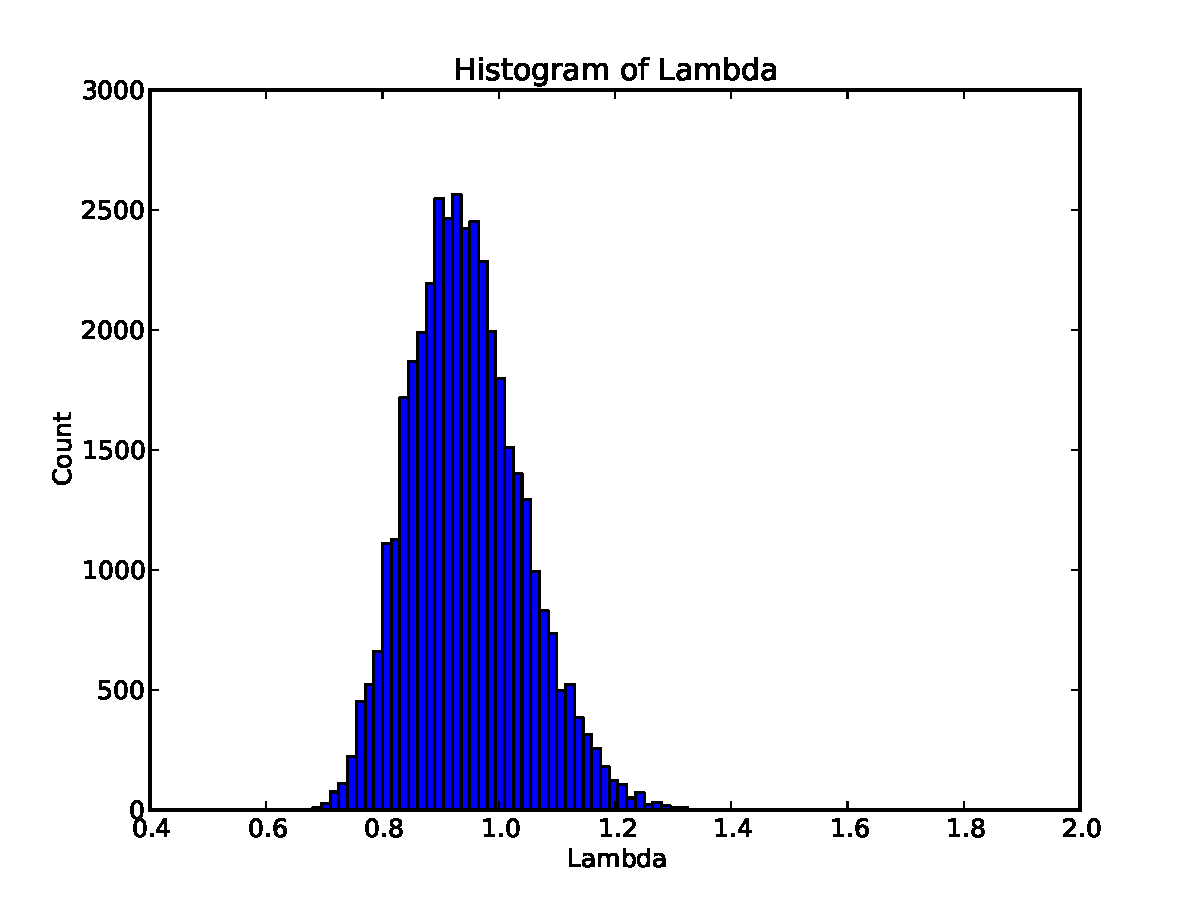
\includegraphics[width=\linewidth]{../ch5-hierarchical.pdf}
\caption{Posterior PDF of the noise standard deviation parameter $\lambda$.}
\label{fig:histogram}
\end{figure}

The histogram shows the support of the data for a range of $\lambda$ values. 
Clearly there is information in the data on the likely values of noise.
Where is the peak of the histogram ? How does this compare to the ratio of the estimated
to true $\sigma$? Usually the ability of the data to constrain noise parameters will trade-off 
with the model complexity given, in this case, by the order of the polynomial.
You can edit the script by changing the estimated noise and rerun to see what happens.

\end{document}

